\subsubsection{\large{Сервис запуска математических методов}}
\addcontentsline{toc}{subsubsection}

Верхнеуровневая архитектура сервиса запуска математических методов представлена на диаграмме компонент
(см. рис\ \ref{pic:architecture__executor-component}).

\begin{figure}[H]
	\hspace*{-2.5 cm}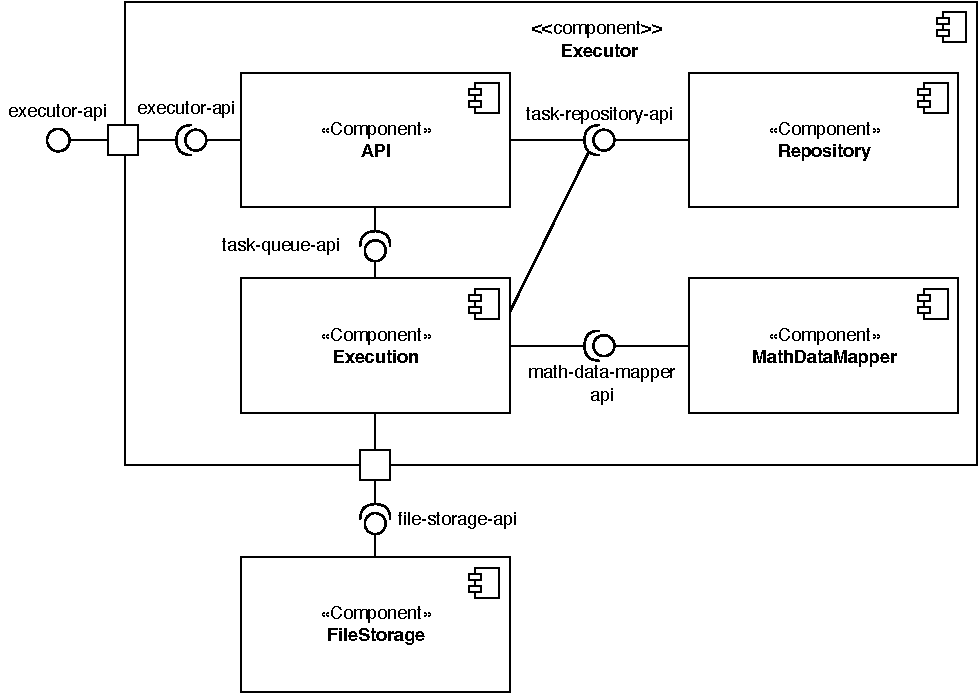
\includegraphics[width=\textwidth]{architecture/pictures/executor/component_common}
	\caption{Верхнеуровневая диаграмма компонент сервиса запуска математических методов}
	\label{pic:architecture__executor-component}
\end{figure}
\vskip 5 mm

Сервис представлен следующими компонентами:
\begin{enumerate}
	\item {
		\textbf{API} -- отвечает за предоставление REST API и отправки задачи в очередь.
	}
	\item {
		\textbf{Repository} -- отвечает за получение и сохранение данных.
	}
	\item {
		\textbf{MathDataMapper} -- отвечает преобразование расчётной модели данных в модель данных математических методик.
	}
	\item {
		\textbf{Execution} -- отвечает за запуск математических методов в отдельном процессе.
	}
\end{enumerate}

Самой технически сложной частью сервиса является компонент, отвечающий за запуск математических методов
в отдельном процессе. Детальное изображение его компонентов представлено
на диаграмме ниже (см. рис\ \ref{pic:architecture__executor-component}).

\begin{figure}[H]
	\hspace*{-2.5 cm}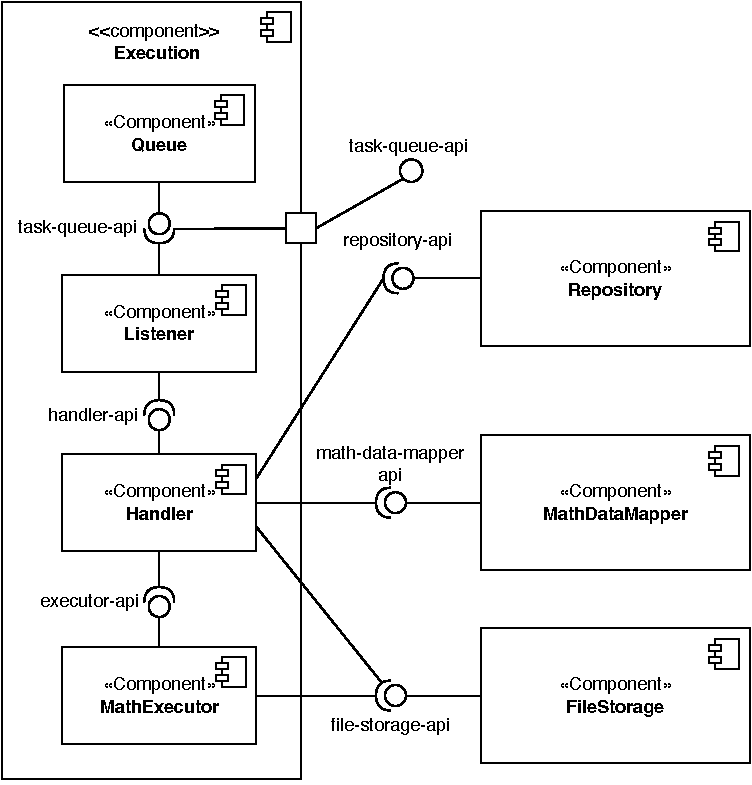
\includegraphics[width=0.8\textwidth]{architecture/pictures/executor/component_detailed}
	\caption{Диаграмма компонента запуска математических методов}
	\label{pic:architecture__executor-detailed-component}
\end{figure}
\vskip 5 mm